%!TEX root = ../main.tex

%=============================================================================== 
%
%    Chapter: vectors
%
%=============================================================================== 

\chapter{Vectors}
\label{chapter:vectors}

In this chapter we'll learn how to manipulate multi-dimensional objects called vectors.						\index{vector|textbf}
Vectors are the precise way to describe directions in space.
We need vectors in order to describe physical quantities like forces, velocities, and accelerations.

Vectors are built from ordinary numbers,
which form the \emph{components} of the vector.
You can think of a vector as a list of numbers,
and \emph{vector algebra} as operations
performed on the numbers in the list.
Vectors can also be manipulated as geometric objects,
represented by arrows in space.
For instance, the arrow that corresponds to the vector $\vec{v}=(v_x,v_y)$ starts at the origin $(0,0)$
and ends at the point $(v_x,v_y)$.
The word vector comes from the Latin \emph{vehere},
which means \emph{to carry}.
Indeed, the vector $\vec{v}$ takes the point $(0,0)$ and carries it to the point $(v_x,v_y)$.

\begin{figure}[H]
	\centering
	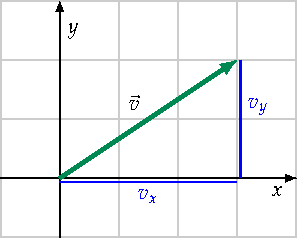
\includegraphics[width=0.4\textwidth]{figures/vectors/vector_components.pdf}
	\vspace{-2mm}
	\caption{	The vector $\vec{v}=(3,2)$ is an arrow in the Cartesian plane.
			The horizontal component of $\vec{v}$ is $v_x=3$
			and the vertical component  is $v_y=2$.}
	\label{fig:vector_components}
\end{figure}




